\documentclass{beamer}
\usetheme{Boadilla}
\usepackage{graphicx}
\usepackage{multicol}
\graphicspath{ {./images} }

\title {Atividade 2 IHC}
\subtitle {Exemplos de Design}
\author {Henrique Tsuyoshi Yara N° 11796083 \\ 
        Gustavo Tsuyoshi Ariga N° 11857215}
\institute {USP - Universidade de São Paulo}

\begin{document}

\begin{frame}{\titlepage}
\end{frame}

\begin{frame}{Índice}
\begin{multicols}{2}
  \tableofcontents
\end{multicols}
\end{frame}

\section{Cognição}
\subsection{Cognição Experimental}
\subsubsection{Comandos comuns}

\begin{frame}{Comandos parecidos Exemplo Ruim}

Processo cognitivo: Memória, Raciocínio

Conceito: Cognição experimental

\begin{itemize}
    \item Para instalar pacotes no Sistema Operacional Linux é necessário o uso de Package Managers, mas tomando de exemplo o pacman da distribuição Arch ele usa um formato não trivial para pesquisar pacotes 
\end{itemize}
\begin{figure}
    \centering
    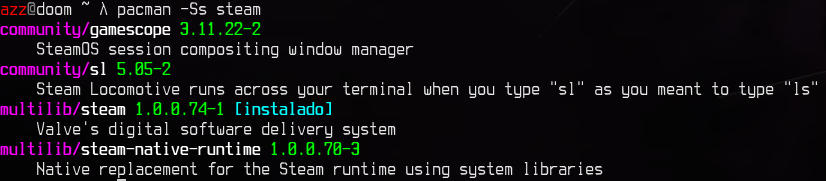
\includegraphics[scale=0.4]{images/Pacman-search.png}
    \caption{Pesquisar o pacote steam no pacman}
\end{figure}

\end{frame}

\begin{frame}{Comandos parecidos Exemplo Bom}

Processo cognitivo: Memória, Raciocínio

Conceito: Cognição experimental

\begin{itemize}
    \item Alguns gerenciadores de pacotes como: apt, dnf, flatpak, etc... Usam um padrão parecido para realizar seus comandos. Por exemplo para pesquisar um pacote no apt: apt search pacote; Para pesquisar um pacote no flatpak: flatpak search pacote. Sendo assim de uma forma mais intuitiva para o usuário
\end{itemize}
\begin{figure}
    \centering
    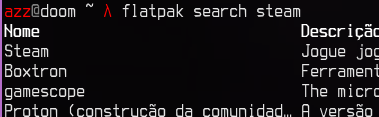
\includegraphics[scale=0.8]{images/Flatpak-Good-Search.png}
    \caption{Pesquisar o pacote steam no flatpak}
\end{figure}

\end{frame}

\subsection{Cognição Reflexiva}
\subsubsection{Mensagem de Erro}

\begin{frame}{Mensagem de Erro Exemplo Ruim}

Processo cognitivo: Raciocínio

Conceito: Cognição Reflexiva

\begin{itemize}
    \item O programa usado foi o xwinwrap e o comando executado estava errado e não conseguiu ser executado, apesar disso o xwinwrap não foi capaz de retornar nenhum log ou erro de por quê o comando não conseguiu ser executado corretamente, ao invés de explicar o problema ele apenas nos retornou o manual do programa
\end{itemize}
\begin{figure}
    \centering
    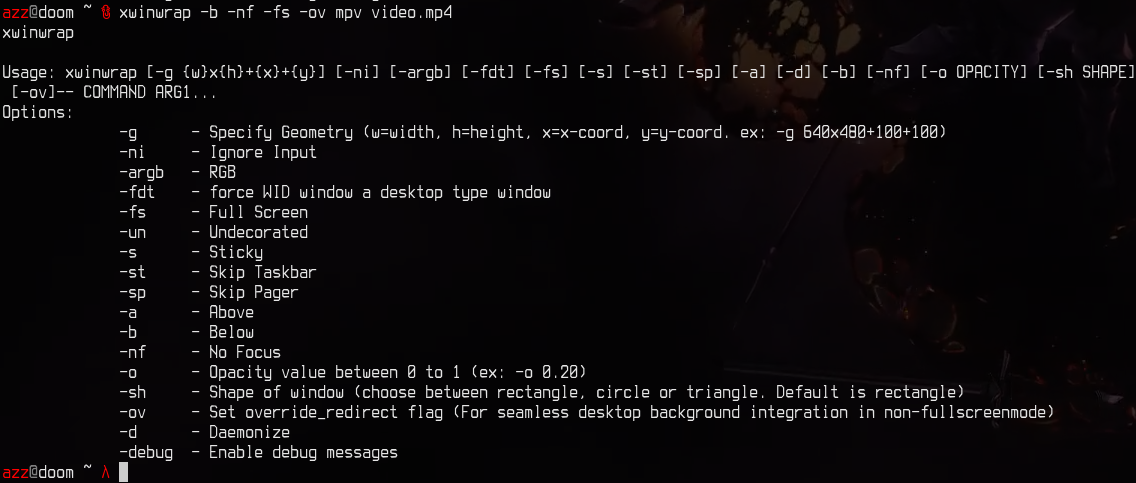
\includegraphics[scale=0.25]{images/xwinwrap-error.png}
    \caption{Comando errado para fixar o programa mpv na área de trabalho}
\end{figure}

\end{frame}

\begin{frame}{Mensagem de Erro Exemplo Bom}

Processo cognitivo: Raciocínio

Conceito: Cognição Reflexiva

\begin{itemize}
    \item O comando usado foi ls em uma pasta não existente, o programa retornou o motivo do progama não conseguir executar corretamente
\end{itemize}
\begin{figure}
    \centering
    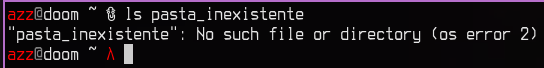
\includegraphics[scale=0.6]{images/ls-error.png}
    \caption{Tentar listar uma pasta não existente com o programa ls}
\end{figure}

\end{frame}

\section{Percepção}
\subsection{Estruturas e Padrões Familiares}
\subsubsection{Botão Registar-se}

\begin{frame}{Botão Registrar-se Exemplo Ruim}

Processo cognitivo: Visão

Conceito: Estruturas e Padrões familiares

\begin{itemize}
    \item Essa tela foi escolhida, pois nela é possível perceber que não existe um botão de registar conta, dessa forma ela não segue o padrão esperado de uma tela de login
\end{itemize}
\begin{figure}
    \centering
    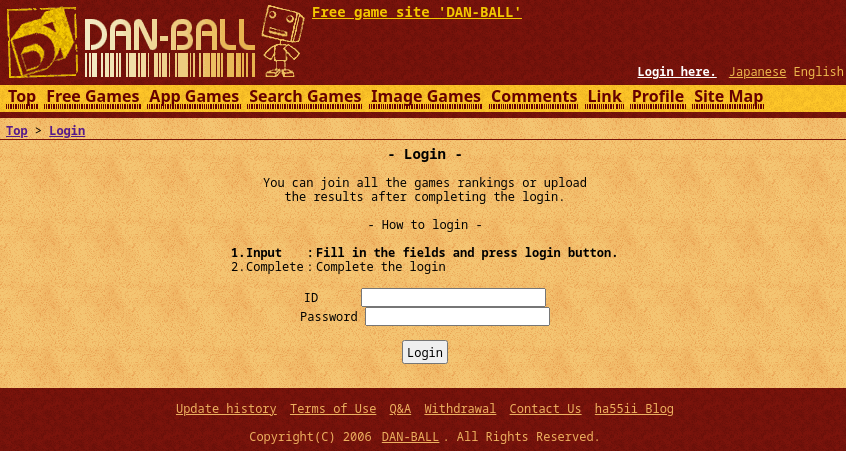
\includegraphics[scale=0.3]{images/Dan-Ball-Login.png}
    \caption{Site de jogos grátis DAN-BALL}
\end{figure}

\end{frame}

\begin{frame}{Botão Registrar-se Exemplo Bom}

Processo cognitivo: Visão

Conceito: Estruturas e Padrões familiares

\begin{itemize}
    \item Nessa tela de login do facebook é fácil encontrar o botão para criar uma conta e fazer login
\end{itemize}
\begin{figure}
    \centering
    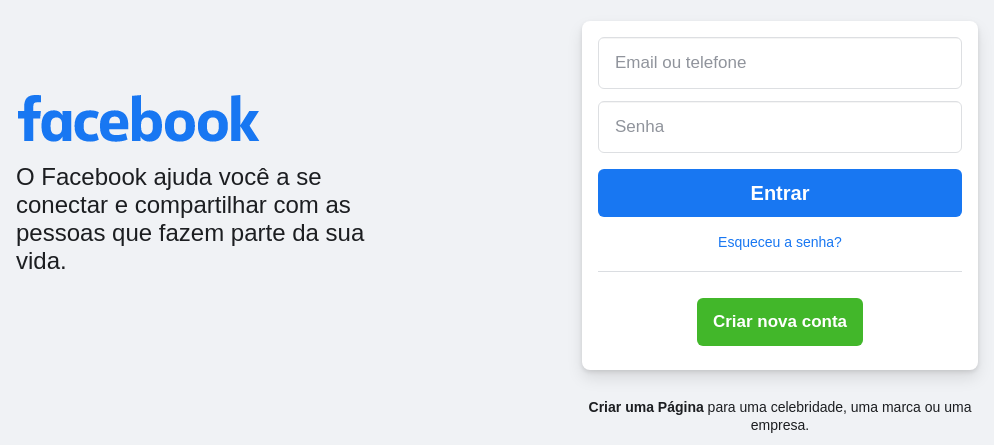
\includegraphics[scale=0.3]{images/Facebook-Login.png}
    \caption{Rede social Facebook}
\end{figure}

\end{frame}

\subsection{Percepção de cores}
\subsubsection{Package Manager}

\begin{frame}{Package Manager Exemplo Ruim}

Processo cognitivo: Visão

Princípio: Percepção de cores

\begin{itemize}
    \item Por mais que o flatpak mostre todas as informações que o usuário necessita, o terminal do usuário acaba ficando muito poluído
\end{itemize}
\begin{figure}
    \centering
    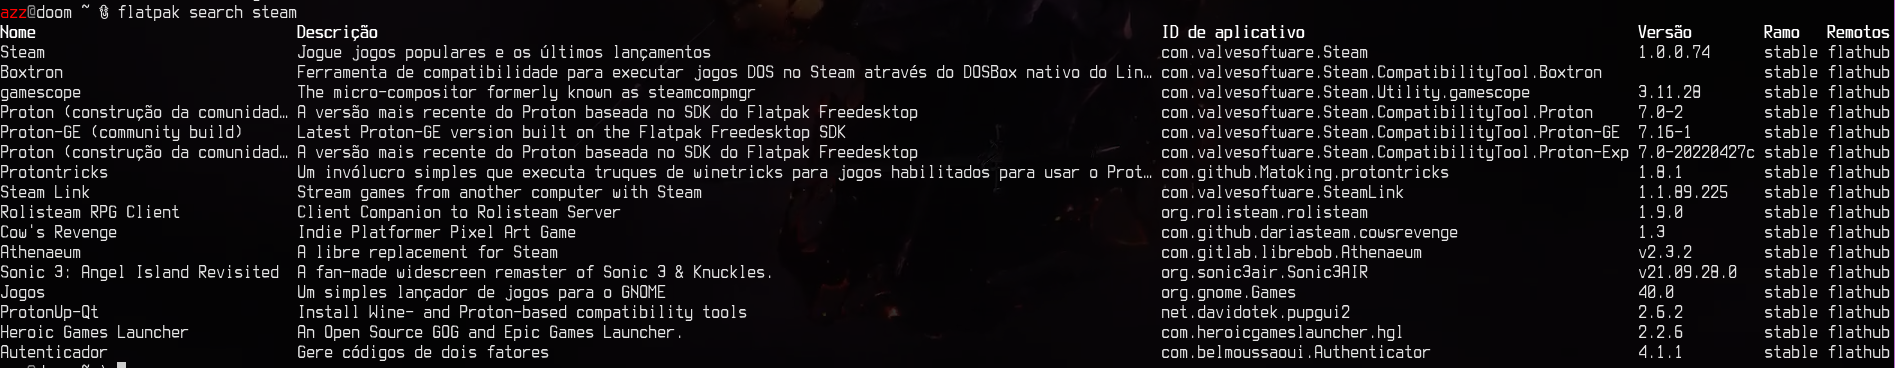
\includegraphics[scale=0.2]{images/Flatpak-Search.png}
    \caption{Pesquisar o pacote steam no flatpak}
\end{figure}

\end{frame}

\begin{frame}{Package Manager Exemplo Bom}

Processo cognitivo: Visão

Princípio: Percepção de cores

\begin{itemize}
    \item O pacman não tem todas as informações para o usuário, mas em questão de guiar a atenção do usuário ele é muito bom! Para quem está acostumado com o pacman é fácil distinguir o nome do pacote, a versão, a descrição e de qual repostório ele está vindo. As cores são essenciais também para facilitar a leitura do usuário
\end{itemize}
\begin{figure}
    \centering
    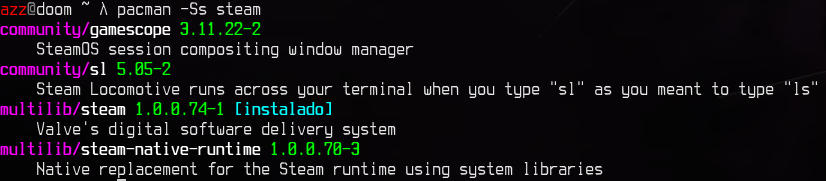
\includegraphics[scale=0.5]{images/Pacman-search.png}
    \caption{Pesquisar o pacote steam no pacman}
\end{figure}

\end{frame}

\subsection{Implementações para o design}
\subsubsection{Usar Ícones}
\begin{frame}{Não Usar Ícones Exemplo Ruim}

Processo cognitivo: Visão

Recomendação: Use imagens onde for possível para indicar uma função/ação

\begin{itemize}
    \item Não usar os ícones para representar alguma informação faz com que o usuário tenha que ler a palavra inteira que ele procura
\end{itemize}
\begin{figure}
    \centering
    
\includegraphics[scale=0.3]{images/casa-dos-filtros.png}
    \caption{Página inicial da casa dos filtros}
\end{figure}

\end{frame}

\begin{frame}{Usar ìcones Exemplo Bom}

Processo cognitivo: Visão

Recomendação: Use imagens onde for possível para indicar uma função/ação

\begin{itemize}
    \item Com a utilização de ícones fica muito mais fácil para o usuário conseguir se localizar no site de forma rápida
\end{itemize}
\begin{figure}
    \centering
    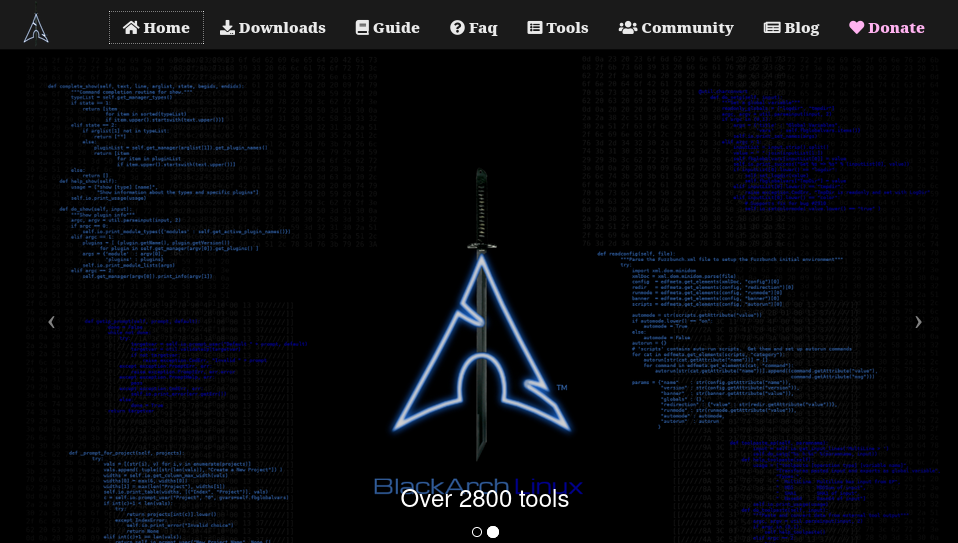
\includegraphics[scale=0.3]{images/black-arch-install.png}
    \caption{Página inicial da distribuição black-arch}
\end{figure}

\end{frame}

\subsubsection{Visibilidade dos Ícones}
\begin{frame}{Visibilidade dos Ícones Exemplo Ruim}

Processo cognitivo: Visão

Princípio: As informações representadas precisam ser perceptíveis e reconhecíveis

\begin{itemize}
    \item Por mais que essa página consiga representar suas opções com ícones, os ícones são muito pequenos e o usuário precisa se esforçar para conseguir identificar os ícones
\end{itemize}
\begin{figure}
    \centering
    
\includegraphics[scale=0.3]{images/hareia-icones.png}
    \caption{Página inicial da Hareia}
\end{figure}

\end{frame}

\begin{frame}{Visibilidade dos Ícones Exemplo Bom}

Processo cognitivo: Visão

Princípio: As informações representadas precisam ser perceptíveis e reconhecíveis

\begin{itemize}
    \item Nessa página é possível ver e reconhecer os ícones mais facilmente, assim facilitando para as pessoas que tem problema de visão ou dificudade na vista
\end{itemize}
\begin{figure}
    \centering
    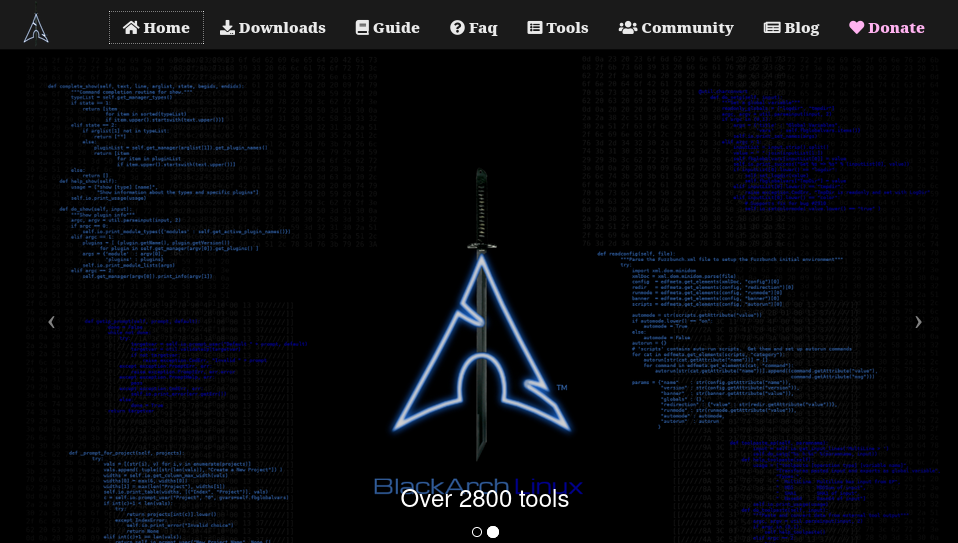
\includegraphics[scale=0.25]{images/black-arch-install.png}
    \caption{Página inicial da distribuição black-arch}
\end{figure}

\end{frame}
\subsubsection{Ações do usuário}
\begin{frame}{Ações do usuário Exemplo Ruim}

Processo cognitivo: Visual

Recomendação: Deixe claro para o usuário o efeito de suas ações

\begin{itemize}
    \item O vi/vim/neovim são um editor de texto  que não são muito triviais para as pessoas que nunca usaram ou leram o manual antes 
\end{itemize}
\begin{figure}
    \centering
    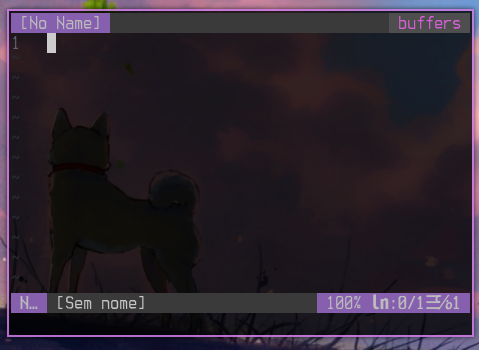
\includegraphics[scale=0.4]{images/vim.png}
    \caption{Neovim aberto}
\end{figure}

\end{frame}

\begin{frame}{Ações do usuário Exemplo Bom}

Processo cognitivo: Visual

Recomendação: Deixe claro para o usuário o efeito de suas ações

\begin{itemize}
    \item O nano é um editor de texto que possui alguns comandos exibidos na sua parte de baixo, assim é possível o usuário que nunca teve contato aprender um pouco de seu funcionamento e também saber qual o resultado de suas ações
\end{itemize}
\begin{figure}
    \centering
    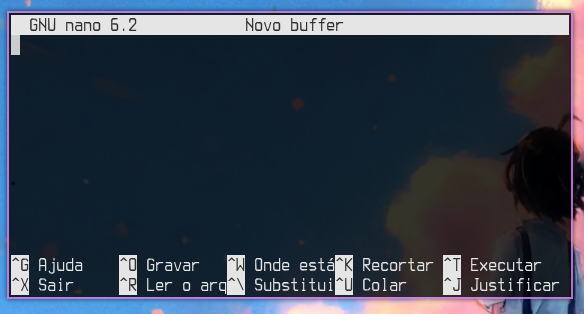
\includegraphics[scale=0.4]{images/nano.png}
    \caption{Nano aberto}
\end{figure}

\end{frame}


\subsubsection{Visualisador de Arquivos}
\begin{frame}{Visualisador de Arquivos Exemplo Ruim}

Processo cognitivo: Visão, Raciocínio

Recomendação: Ver e escolher ou ouvir e escolher é mais fácil do que lembrar e digitar

\begin{itemize}
    \item O ranger é uma ferramenta no terminal do usuário feito para o usuário conseguir navegar e organizar seus arquivos. Mas é uma ferramenta controlada pelo terminal e não tem nenhuma explicação de o que está acontecendo na tela da esquerda (Diretório pai), na tela do meio (Diretório atual) e na tela da direita (Arquivo Selecionado).
\end{itemize}
\begin{figure}
    \centering
    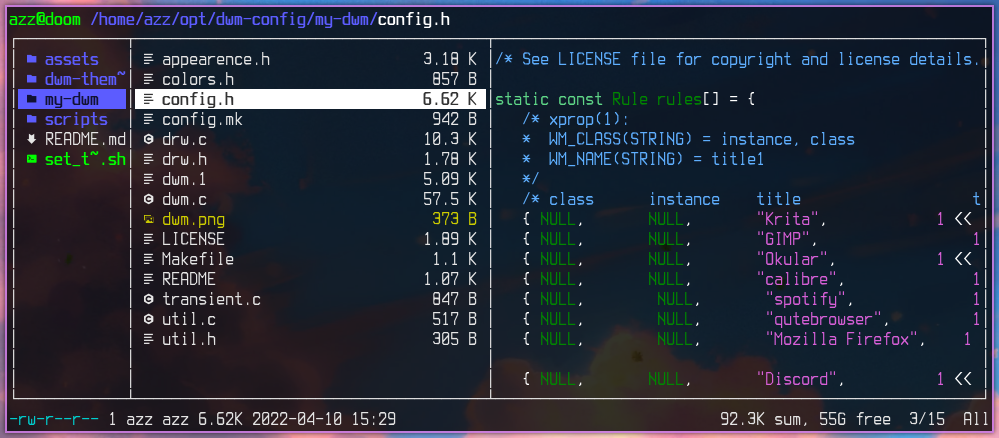
\includegraphics[scale=0.2]{images/ranger.png}
    \caption{Ranger visualizador de arquivos}
\end{figure}

\end{frame}

\begin{frame}{Visualisador de Arquivos Exemplo Bom}

Processo cognitivo: Visão, Raciocínio

Recomendação: Ver e escolher ou ouvir e escolher é mais fácil do que lembrar e digitar

\begin{itemize}
    \item O dolphin é uma ferramenta para arquivos, nele é possível ver a pasta que estamos atualmente, identificar o tipo de cada arquivo facilmente, graças aos ícones, e com os botões de cima é possível filtrar, organizar e mudar o tipo de visualização! Melhorando a experiência do usuário
\end{itemize}
\begin{figure}
    \centering
    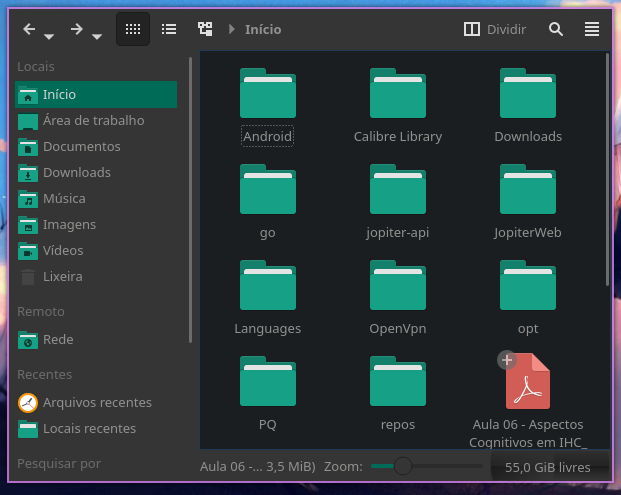
\includegraphics[scale=0.2]{images/dolphin.png}
    \caption{Dolphin visualizador de arquivos}
\end{figure}

\end{frame}

\subsubsection{Organizar Playlists}
\begin{frame}{Organizar Playlists Exemplo Ruim}

Processo cognitivo: Memória, Visão

Recomendação: Permita marcações personalizadas de progresso

\begin{itemize}
    \item  Ao adicionar uma música em uma lista de músicas no spotify, a tela circulada em azul aparece para o usuário escolher a playlist que ele deseja adicionar a música escolhida. O usuário não sabe qual playlist já tem a música selecionada e não consegue adicionar mais de uma lista de música por vez
\end{itemize}
\begin{figure}
    \centering
    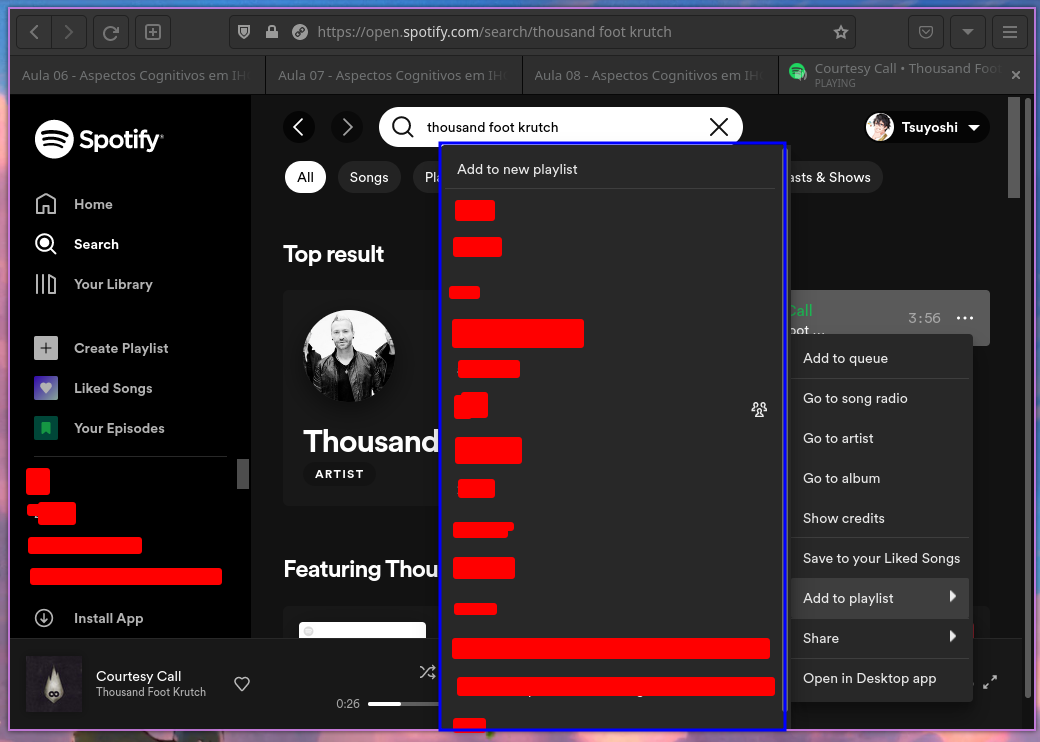
\includegraphics[scale=0.15]{images/spotify-playlist.png}
    \caption{Adicionando músicas nas listas do spotify}
\end{figure}

\end{frame}

\begin{frame}{Organizar Playlists Exemplo Bom}

Processo cognitivo: Memória, Visão

Recomendação: Permita marcações personalizadas de progresso

\begin{itemize}
    \item Ao adicionar um vídeo em uma lista de vídeos no youtube, uma pequena tela com informações sobre quais listas a lista está inserida é mostrada ao usuário, o usuário por sua vez pode escolher mais de uma lista onde quer adicionar sueu vídeo e ainda sabe qual playlist contém seu vídeo
\end{itemize}
\begin{figure}
    \centering
    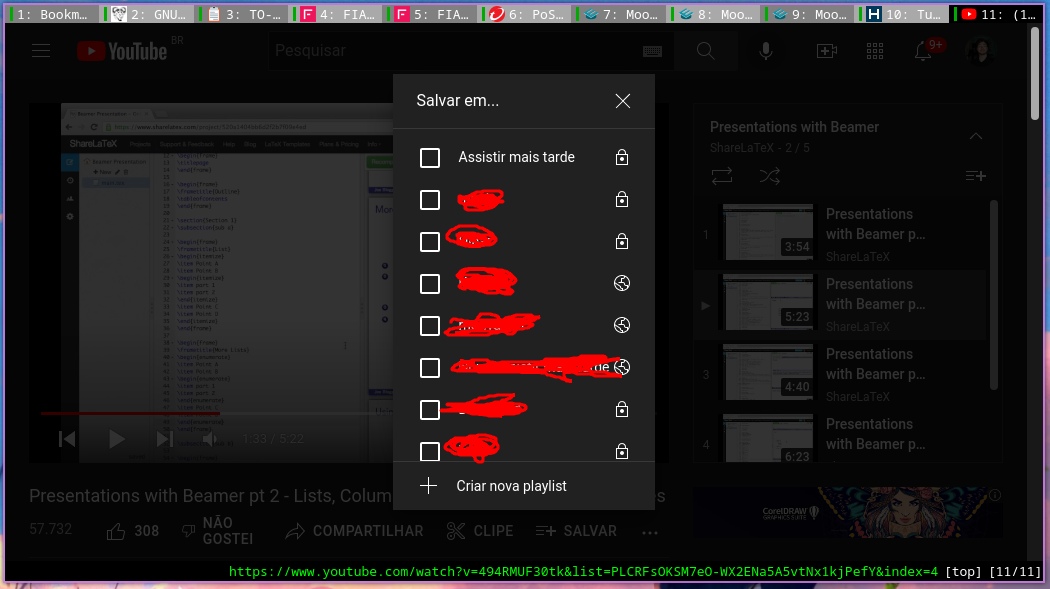
\includegraphics[scale=0.2]{images/youtube-playlist.png}
    \caption{Adicionando vídeos em listas do youtube}
\end{figure}

\end{frame}

\subsubsection{Barra de Progresso}

\begin{frame}{Indique progresso Exemplo Ruim}

Percepção Cognitiva: Visão

Recomendação: Indique progresso

\begin{itemize}
    \item Compactando alguns arquivos usando o programa zip, é possível ver apenas uma porcentagem do lado de cada arquivo que está sendo compactado
\end{itemize}
\begin{figure}
    \centering
    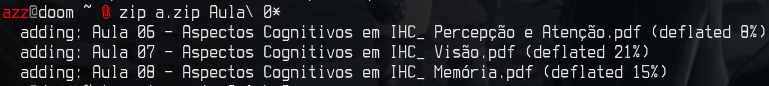
\includegraphics[scale=0.5]{images/unzip.png}
    \caption{Comando zip para compactar}
\end{figure}
\end{frame}

\begin{frame}{Indique progresso Exemplo Bom}

Percepção Cognitiva: Visão

Recomendação: Indique progresso

\begin{itemize}
    \item Atualizando o programa pip3 é possível ver uma barra de progresso, facilitando assim a visualização do progresso por parte do usuário
\end{itemize}
\begin{figure}
    \centering
    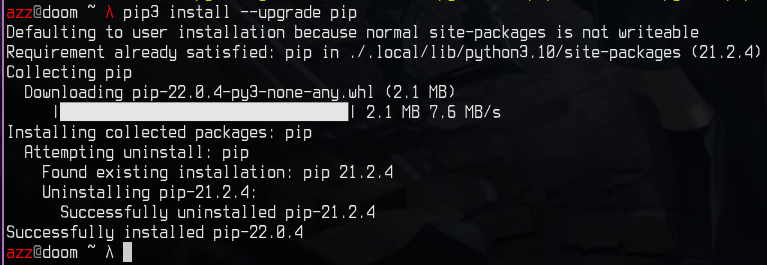
\includegraphics[scale=0.4]{images/python-pip.png}
    \caption{Atualizando o programa pip}
\end{figure}

\end{frame}

\subsubsection{Chunking}

\begin{frame}{Chunking de Informações Exemplo Ruim}

Percepção Cognitiva: Visão, Memória

Recomendação: Chunking ajuda a perceber e entrar dados

\begin{itemize}
    \item Ao tentar editar as informçaões pessoais no perfil do Ali-express é possível notar que o CPF não é formatade de uma forma fácil para o usuário conseguir verificar se a informação está correta
\end{itemize}
\begin{figure}
    \centering
    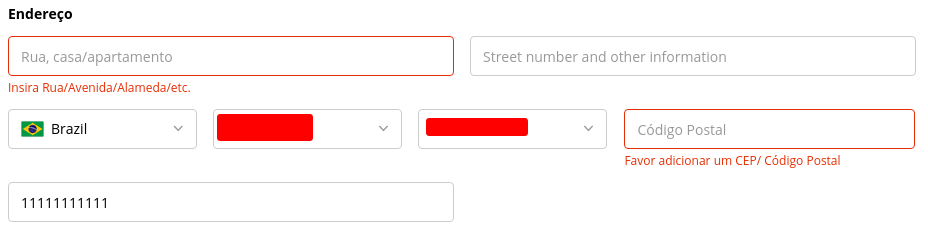
\includegraphics[scale=0.4]{images/Ali-express.png}
    \caption{Edição de CPF no Ali Express}
\end{figure}
\end{frame}

\begin{frame}{Chunking de Informações Exemplo Bom}

Percepção Cognitiva: Visão, Memória

Recomendação: Chunking ajuda a perceber e entrar dados

\begin{itemize}
    \item Em contra partida, ao tentar editar as informações pessoas no site vagas, é possível ver que o CPF é formatado de uma forma que nós estamos acostumados à ler, e dessa forma facilitando a verificação do CPF
\end{itemize}
\begin{figure}
    \centering
    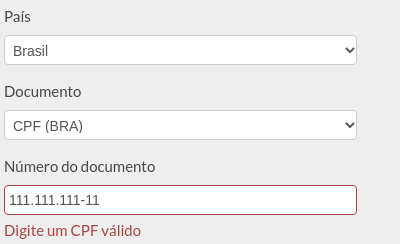
\includegraphics[scale=0.3]{images/Vagas.png}
    \caption{Edição do CPF no Vagas}
\end{figure}

\end{frame}

\subsubsection{Uso de miniaturas}
\begin{frame}{Uso de miniaturas Exemplo Ruim}

Percepção Cognitiva: Visão

Recomendação: Use miniaturas para mostrar imagens de modo mais econômico

\begin{itemize}
    \item No overleaf para poder se locomover no texto existe essa pequena parte para o usuário poder se deslocar facilmente pelo texto
\end{itemize}
\begin{figure}
    \centering
    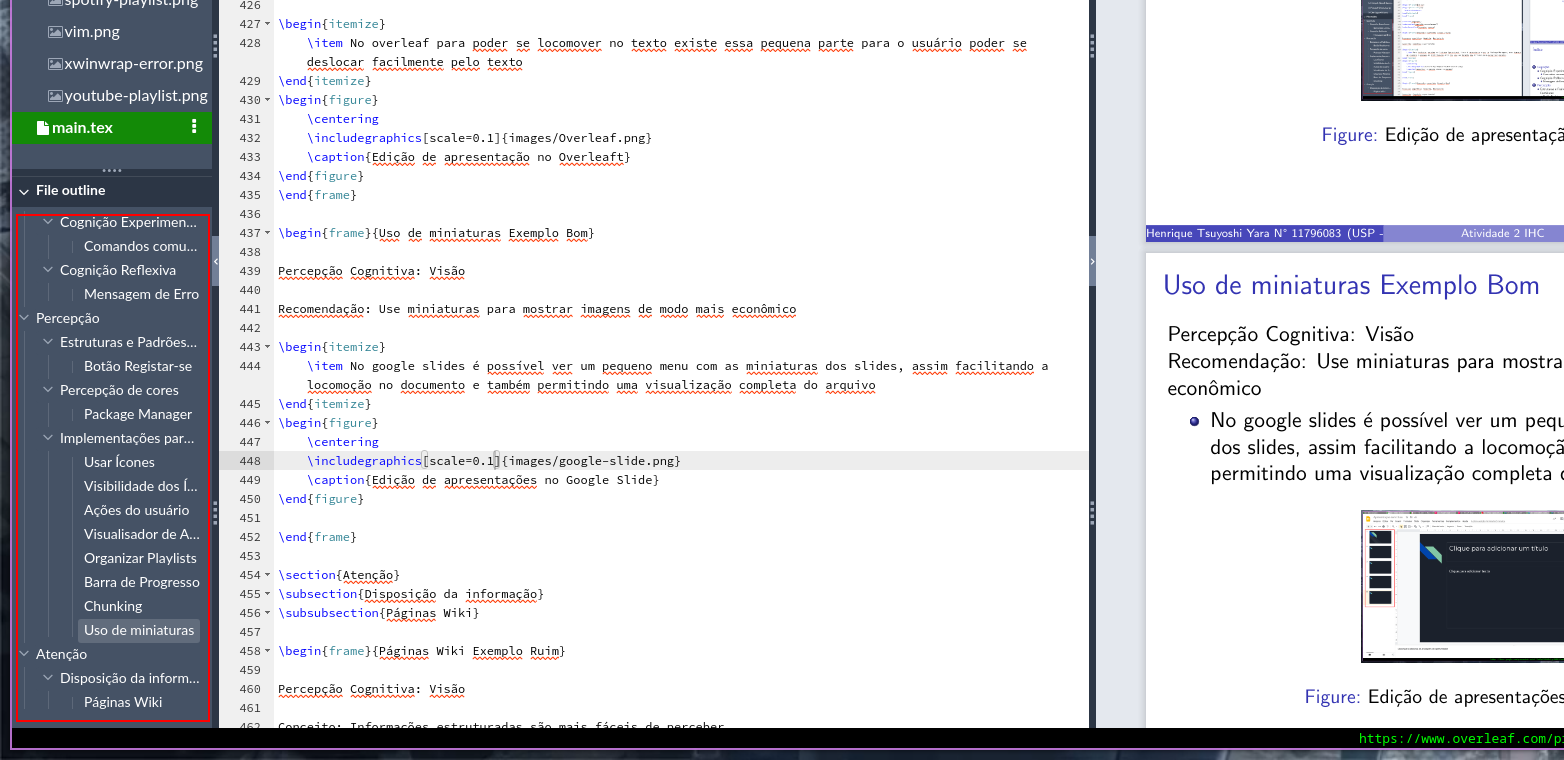
\includegraphics[scale=0.1]{images/Overleaf.png}
    \caption{Edição de apresentação no Overleaf}
\end{figure}
\end{frame}

\begin{frame}{Uso de miniaturas Exemplo Bom}

Percepção Cognitiva: Visão

Recomendação: Use miniaturas para mostrar imagens de modo mais econômico

\begin{itemize}
    \item No google slides é possível ver um pequeno menu com as miniaturas dos slides, assim facilitando a locomoção no documento e também permitindo uma visualização completa do arquivo
\end{itemize}
\begin{figure}
    \centering
    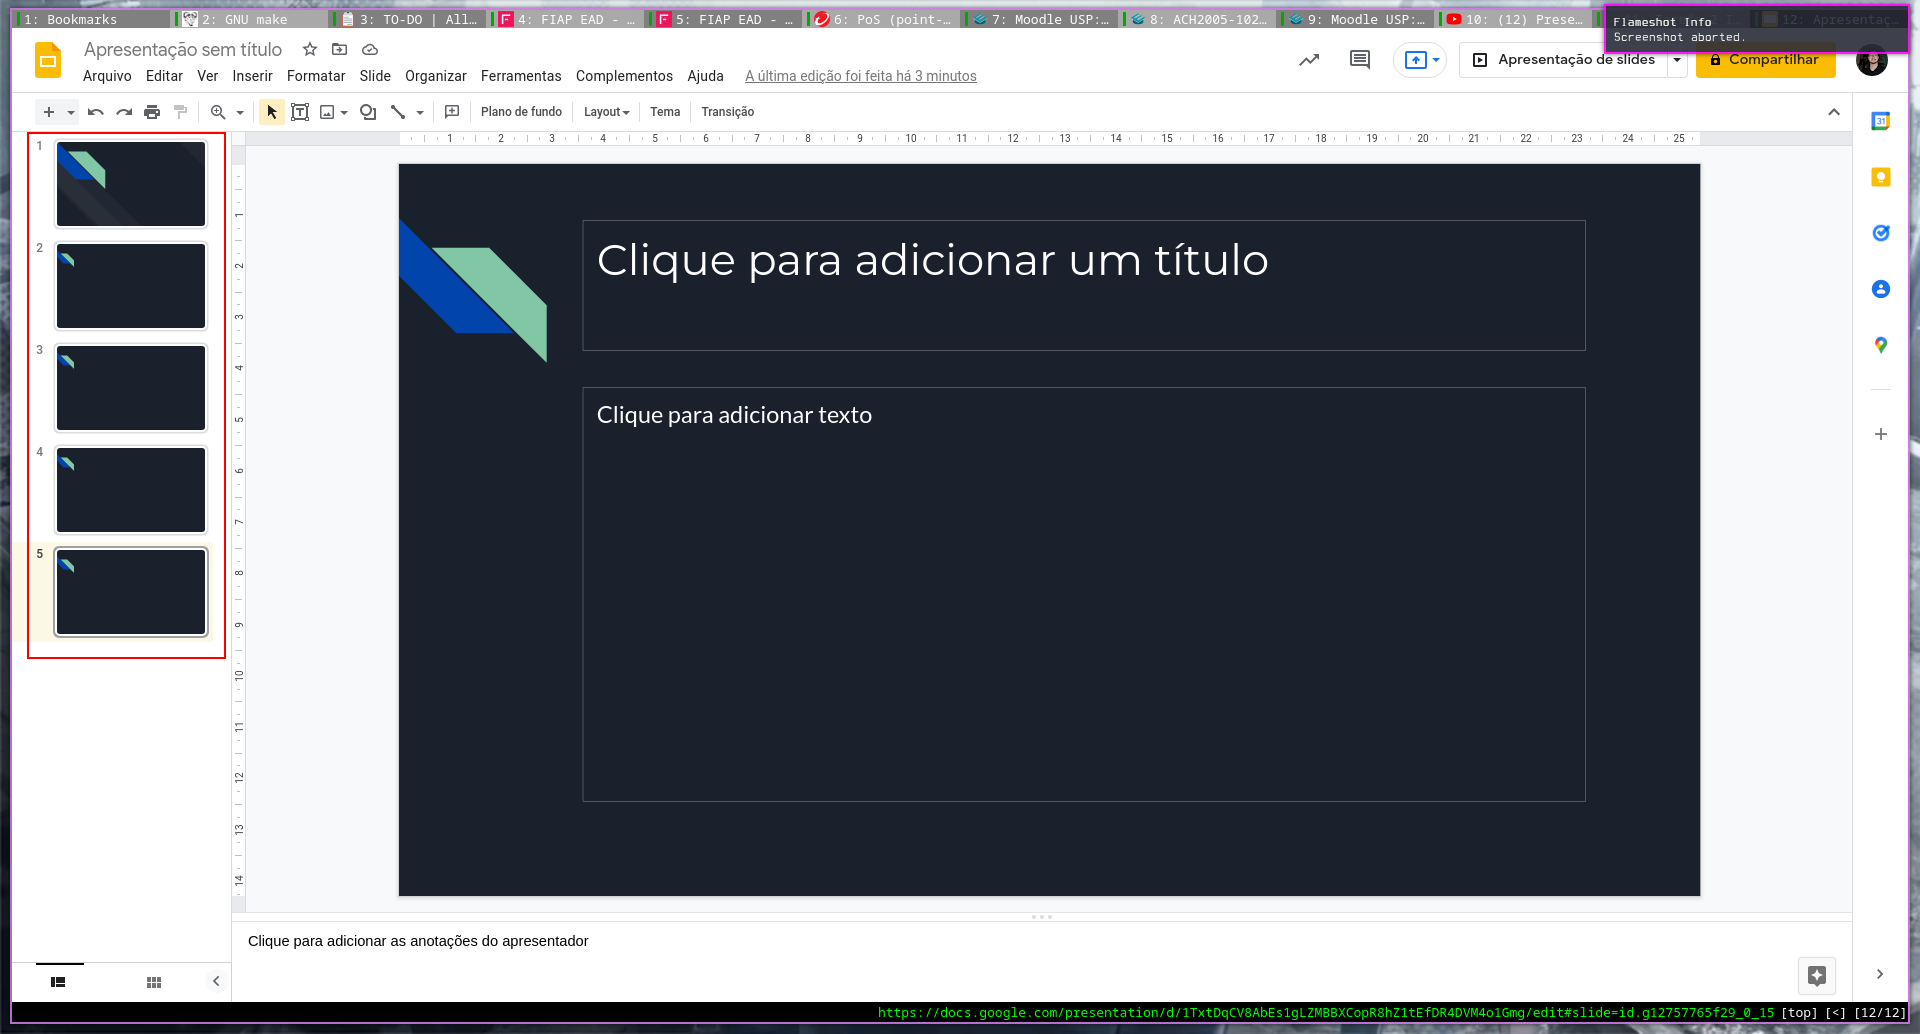
\includegraphics[scale=0.1]{images/google-slide.png}
    \caption{Edição de apresentações no Google Slide}
\end{figure}

\end{frame}

\subsubsection{Alerta sobre tarefas incompletas}
\begin{frame}{Alerta sobre tarefas incompletas Exemplo Ruim}

Percepção Cognitiva: Visão

Recomendação: Alerte o usuário sobre tarefas incompletas

\begin{itemize}
    \item Na tela de registro do project Euler é possível ver mensagens de erros após o usuário tentar se cadastrar
\end{itemize}
\begin{figure}
    \centering
    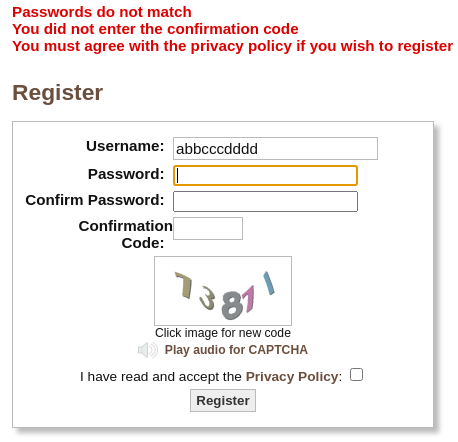
\includegraphics[scale=0.3]{images/Project-Euler.png}
    \caption{Tela de registro Project Euler}
\end{figure}
\end{frame}

\begin{frame}{Alerta sobre tarefas incompletas Exemplo Bom}

Percepção Cognitiva: Visão

Recomendação: Alerte o usuário sobre tarefas incompletas

\begin{itemize}
    \item Aqui podemos ver que o Ali Express notifica o usuário por não ter preenchido certos campos, assim o usuário não perde tempo procurando qual campo ele não preencheu
\end{itemize}
\begin{figure}
    \centering
    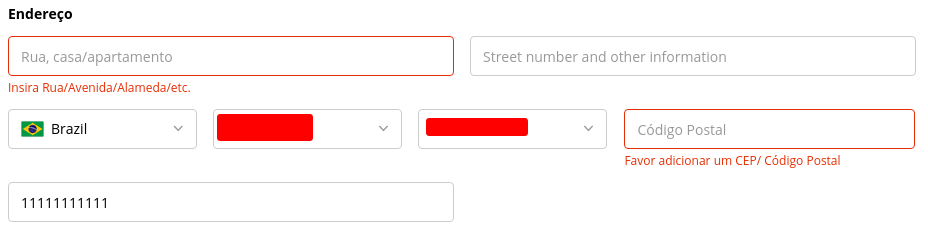
\includegraphics[scale=0.3]{images/Ali-express.png}
    \caption{Edição de CPF no Ali Express}
\end{figure}

\end{frame}


\subsubsection{Limite os indicativos ou chamadas para ação em cada tela/página}
\begin{frame}{Limitar indicativos e chamadas para ação Exemplo Ruim}

Percepção Cognitiva: Visão

Recomendação: Limite os indicativos ou chamadas para ação em cada tela/página

\begin{itemize}
    \item Na tela inicial é possível ver muita informação aglomerada que pode acabar dificultando para os usuários chegarem aos seus objetivos
\end{itemize}
\begin{figure}
    \centering
    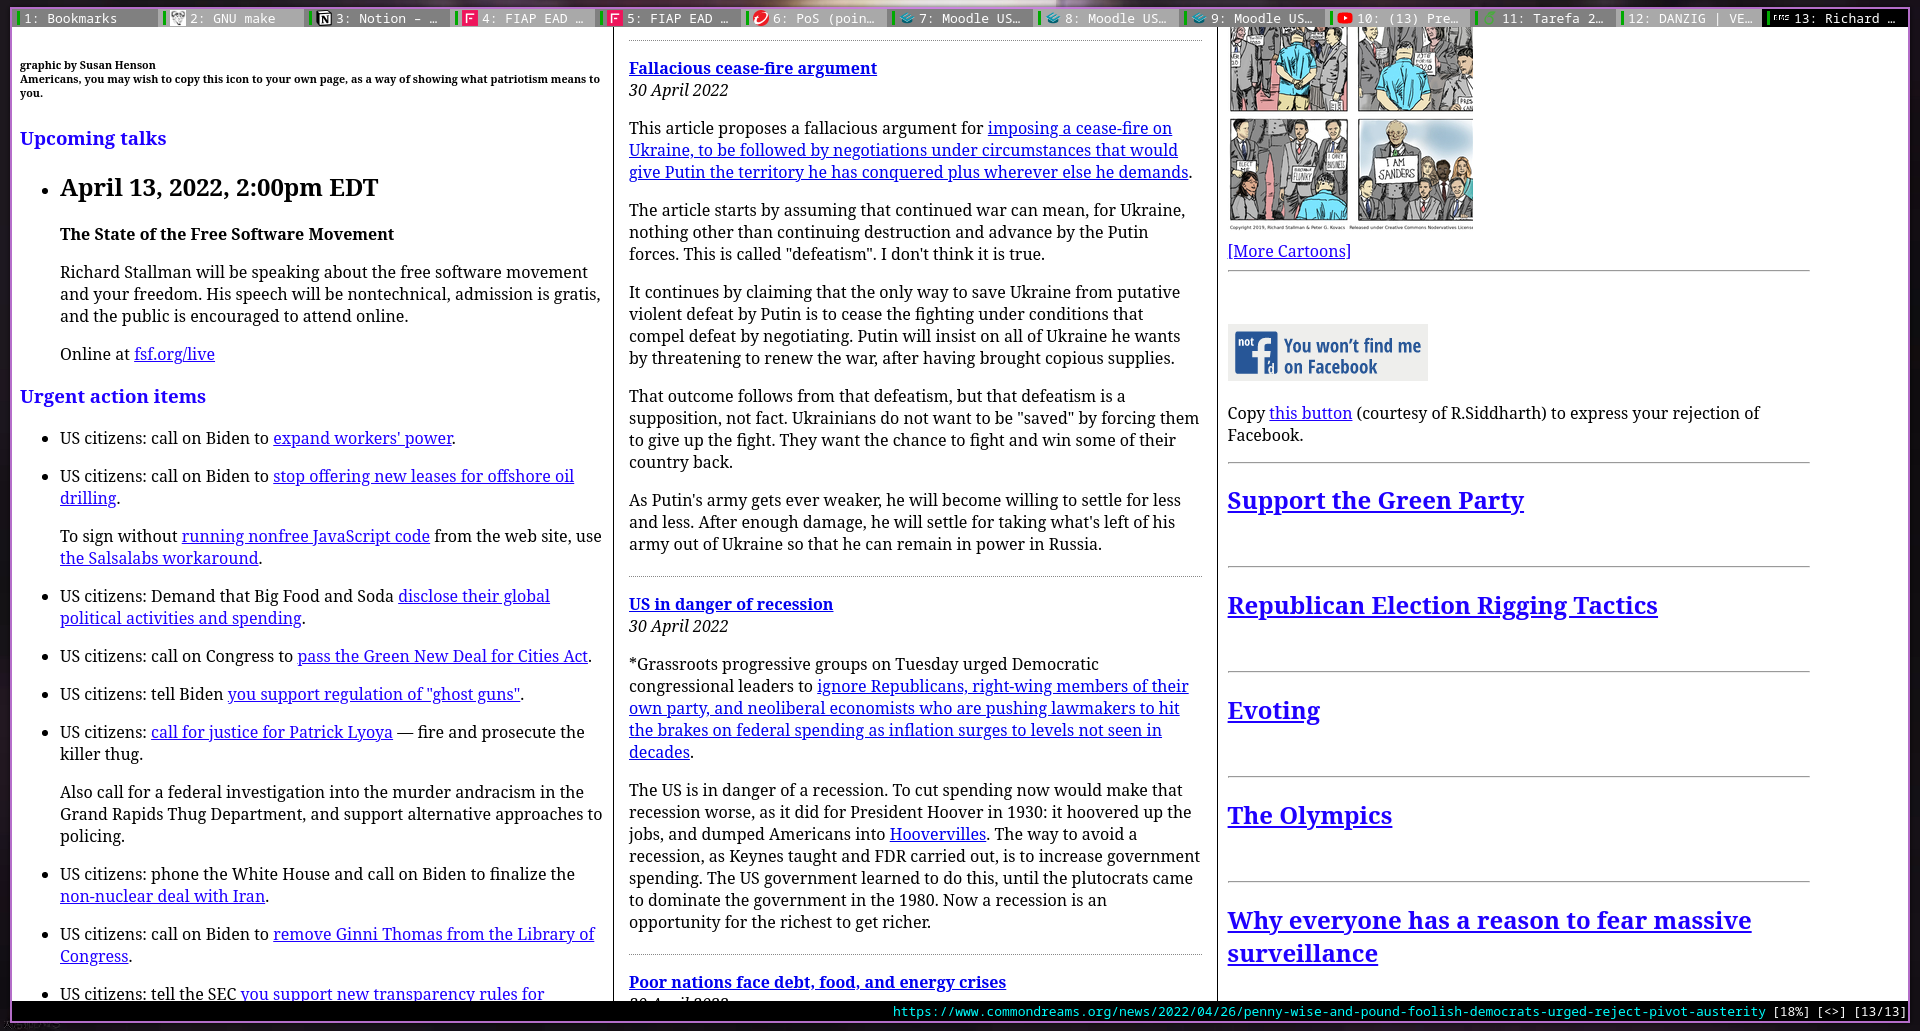
\includegraphics[scale=0.15]{images/rsman.png}
    \caption{Site pessoal do Richard Stallman}
\end{figure}
\end{frame}

\begin{frame}{Limitar indicativos e chamadas para ação Exemplo Bom}

Percepção Cognitiva: Visão

Recomendação: Limite os indicativos ou chamadas para ação em cada tela/página

\begin{itemize}
    \item É possível perceber o menu na esquerda no site pessoal algumas opções para o usuário conseguir se guiar e chegar nas informações que ele deseja
\end{itemize}
\begin{figure}
    \centering
    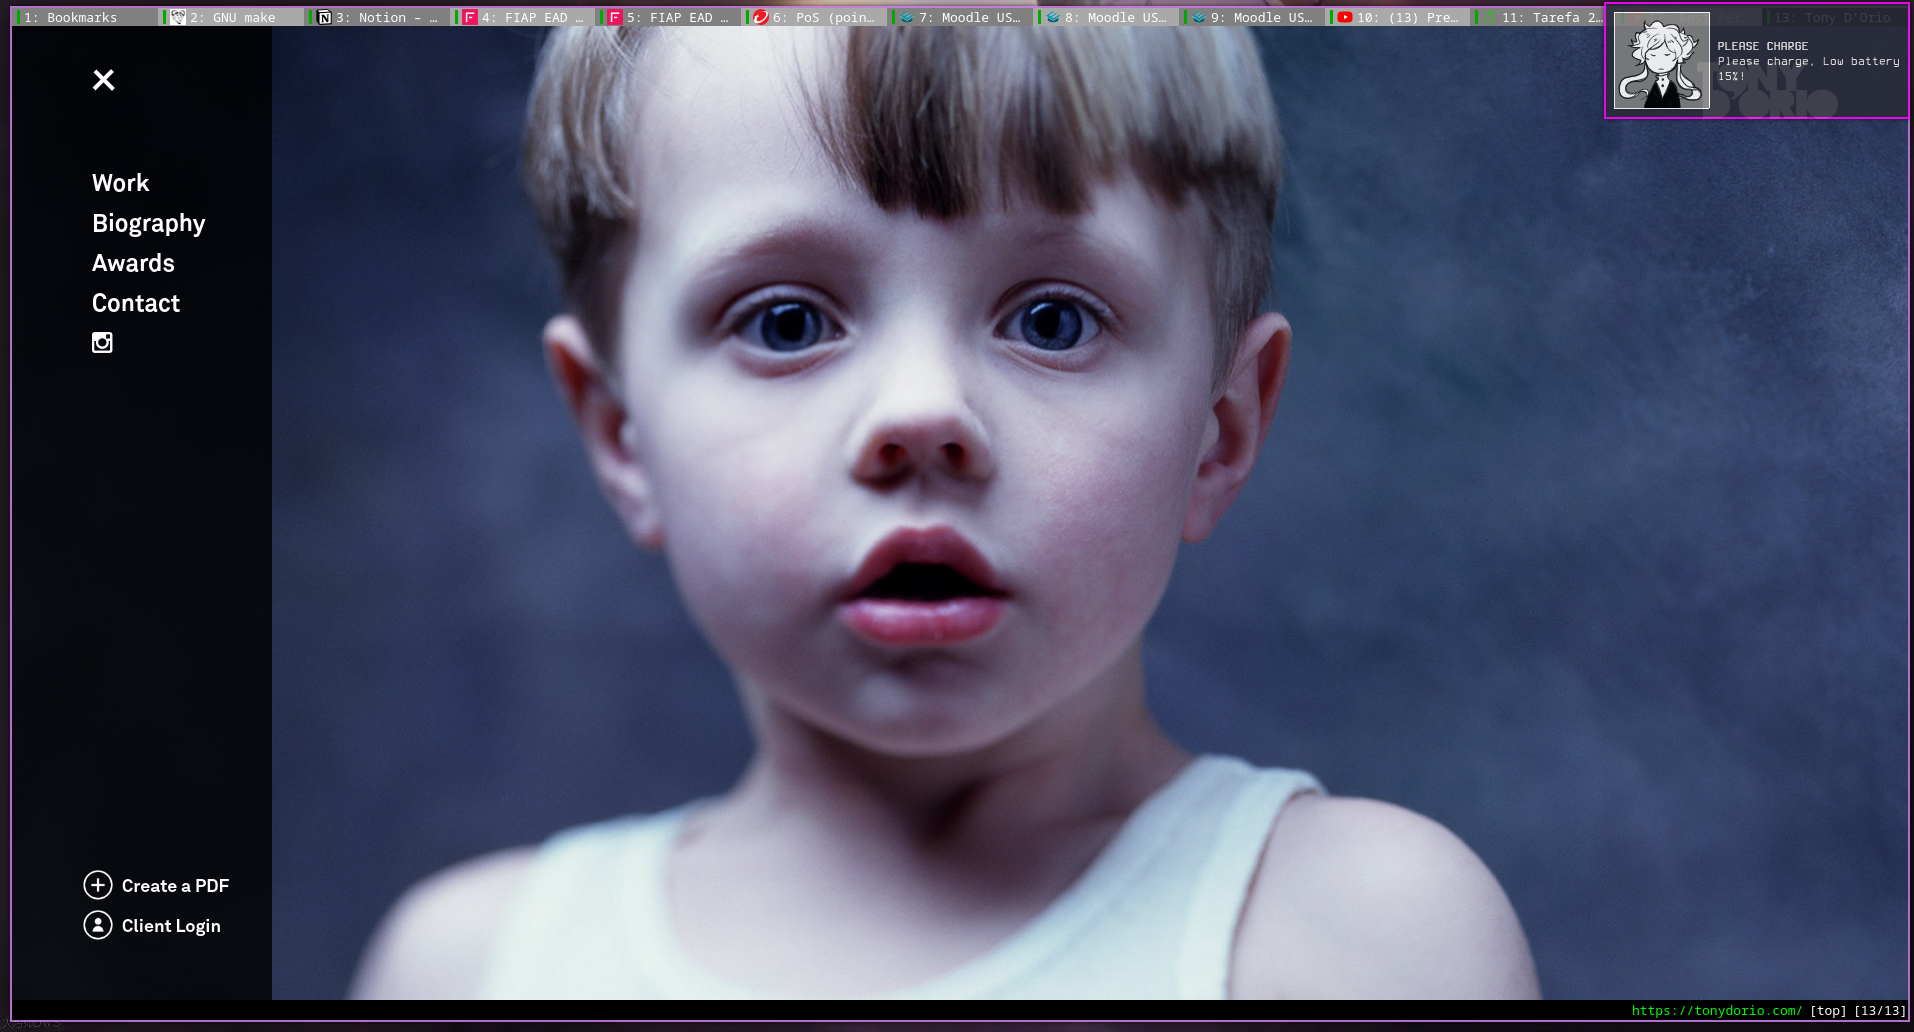
\includegraphics[scale=0.15]{images/Tomd.png}
    \caption{Site pessoal do Tom D'Orio}
\end{figure}

\end{frame}

\section{Atenção}
\subsection{Disposição da informação}
\subsubsection{Páginas Wiki}

\begin{frame}{Páginas Wiki Exemplo Ruim}

Percepção Cognitiva: Visão

Conceito: Informações estruturadas são mais fáceis de perceber

\begin{itemize}
    \item Na wiki do Arch Linux é possível perceber que as informações da barra de navegação não seguem o conteúdo da wiki
\end{itemize}
\begin{figure}
    \centering
    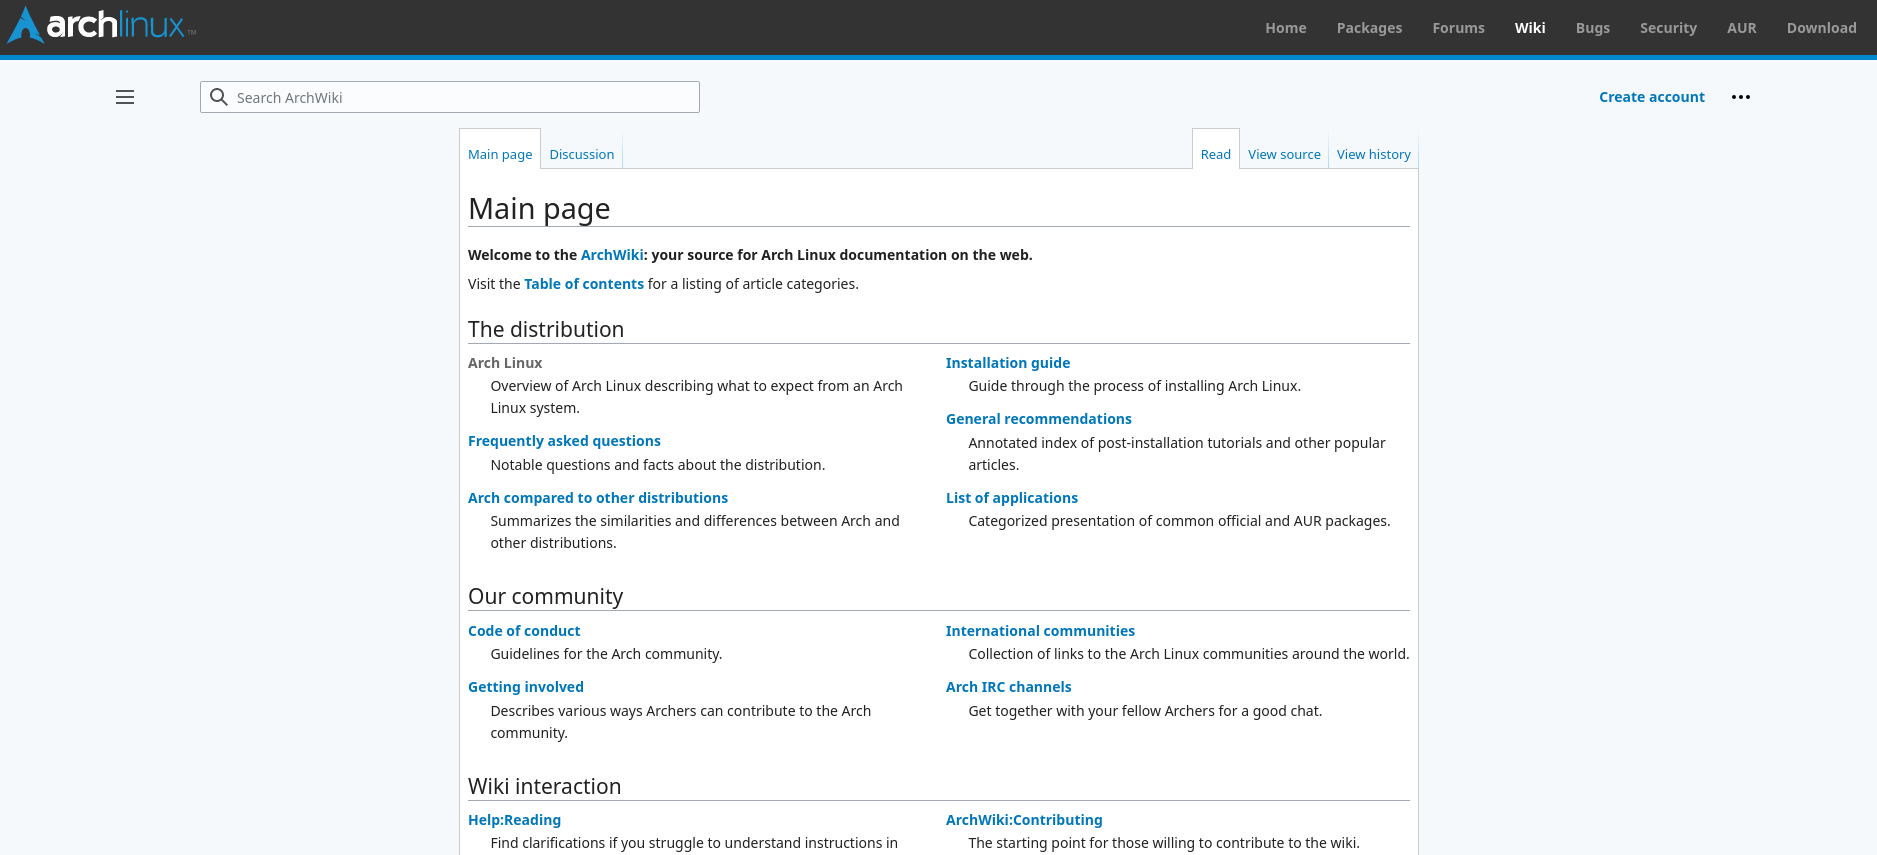
\includegraphics[scale=0.15]{images/Arch-wiki.png}
    \caption{Pagina Wiki da distribuição Arch Linux}
\end{figure}
\end{frame}

\begin{frame}{Páginas Wiki Exemplo Bom}

Percepção Cognitiva: Visão

Conceito: Informações estruturadas são mais fáceis de perceber

\begin{itemize}
    \item Em contra partida a wiki do Gentoo tem as informações mais bem estuturadas no centro da página
\end{itemize}
\begin{figure}
    \centering
    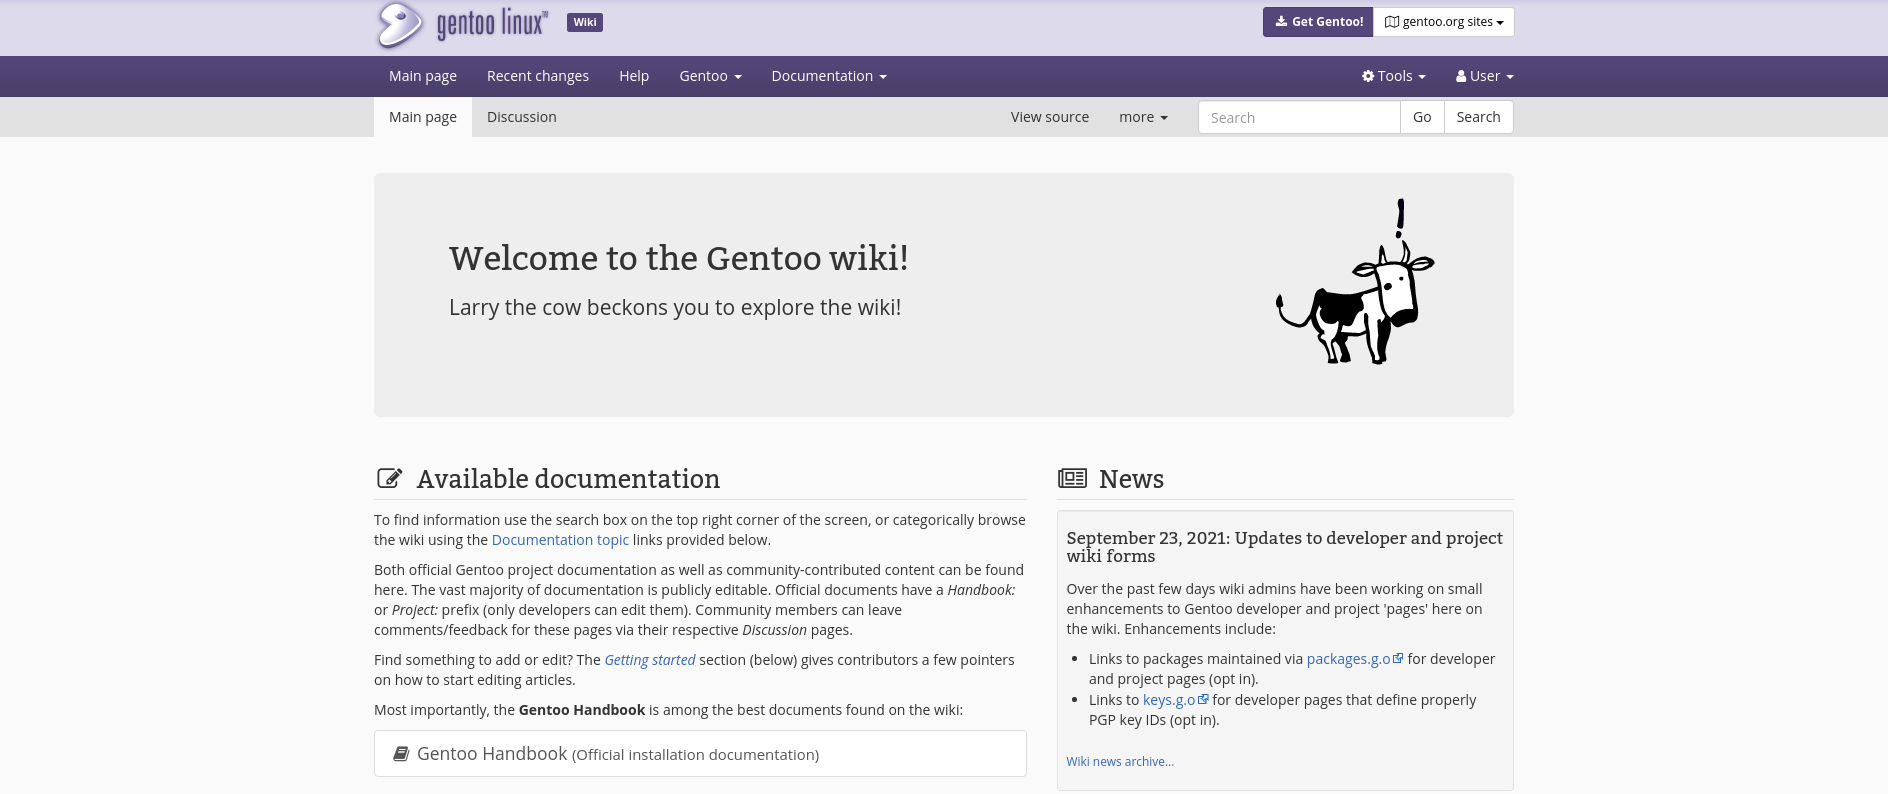
\includegraphics[scale=0.2]{images/Gentoo-wiki.png}
    \caption{Página Wiki da distribuição Gentoo Linux}
\end{figure}

\end{frame}

\end{document}
